
\subsection{The new exact term at side length seven}
An exhaustive run of the unique-longest-edge algorithm rules out 11
points in \(G_7\). It completed all 31 diameter-edge orbits, visiting
60,290,915 recursive search nodes in 525.875 seconds. The original source
snapshot, its SHA-256 digest, the full case log, and the structured result
are included. An independent Python enumeration regenerated all 810
eligible grid edges and their 31 orbits and checked that the log covers
every case with the correct endpoints and squared diameter.

A matching 10-point witness is
\[
\begin{aligned}
A_7=\{&(0,0,0),(2,0,0),(0,6,0),(6,1,2),(4,2,0),\\
      &(6,1,3),(3,6,6),(5,1,5),(6,4,6),(4,5,5)\}.
\end{aligned}
\]
Its 45 pair distances are all distinct. Therefore
\[
\boxed{a_7=10},\qquad
(a_0,\ldots,a_7)=(0,1,3,4,6,7,9,10).
\]
The independent case-coverage check verifies the completeness of the
outer split and the witness arithmetic. The impossibility conclusion
also relies on the correctness of the supplied exhaustive-search
program, whose pruning rules are proved in Section~\ref{sec:algorithm}.
It is a reproducible computer-assisted result, not a claim that a short
hand enumeration or a formally verified proof trace was obtained.

A second complete computation, using a prefix of the four largest
edges together with the later graph pruning, again excluded all 31
cases. It required 5,244,129 calls to the inner clique search and
43.767 seconds. The outer edge-prefix recursion is not included in
that inner-call count. The two implementations share core ideas and
are not wholly independent proof engines, but they use different
complete case refinements and agree on the result. Their recorded
times are observations under shared CPU load.

\subsection{The new exact term at side length eight}
The six-largest-edge prefix algorithm excludes 13 points in \(G_8\).
There are 87 available squared distances. A 13-point set would use
78 of them, so its longest edge must have squared length at least 101.
The 660 eligible grid edges form 23 orbits under the 48 cube
isometries. Every orbit was exhausted, with 38,430,195 calls to the
inner clique search in 445.028 seconds. As above, the node count
excludes calls to the outer edge-prefix recursion. Independent
enumeration checks all orbit representatives, the logged endpoints
and diameters, complete coverage, and the frozen source digest.

The 12-point construction displayed below supplies the matching lower
bound. Consequently,
\[
\boxed{a_8=12},\qquad
(a_0,\ldots,a_8)=(0,1,3,4,6,7,9,10,12).
\]
This computation uses the same audited recursive invariants as the
side-seven search. The archived proof source accepts prefixes up to
six edges; the recursion itself is the same as the version tested
against an independent reference enumerator on small instances.
The validation package distinguishes those finite regression tests
from the mathematical completeness argument and the full side-eight
run.

Further budgeted runs attempted to exclude 15 points at side nine and
17 points at side ten. Both reached approximately 600 seconds with
status \code{UNKNOWN}. The side-nine run completed cases 0 through 8
and stopped during case 9; the side-ten run completed cases 0 through 3
and stopped during case 4. These partial records are retained separately
for reproducibility. They give no improved global upper bound, so the
final intervals remain \(13\le a_9\le15\) and
\(14\le a_{10}\le17\).


\subsection{Explicit improvements at side lengths 8, 9, and 10}
The following point lists use coordinates from 0 through \(n-1\).
Their complete squared-distance inventories are supplied as JSON.
\[
\begin{aligned}
A_8=\{&(7,4,0),(2,0,1),(7,0,0),(0,7,7),\\
      &(2,5,7),(7,3,0),(7,7,7),(1,5,6),\\
      &(4,7,3),(3,1,7),(5,0,0),(4,1,1)\}.
\end{aligned}
\]
The set \(A_8\) has 12 points and 66 distinct squared distances.
\begin{figure}[ht]
\centering
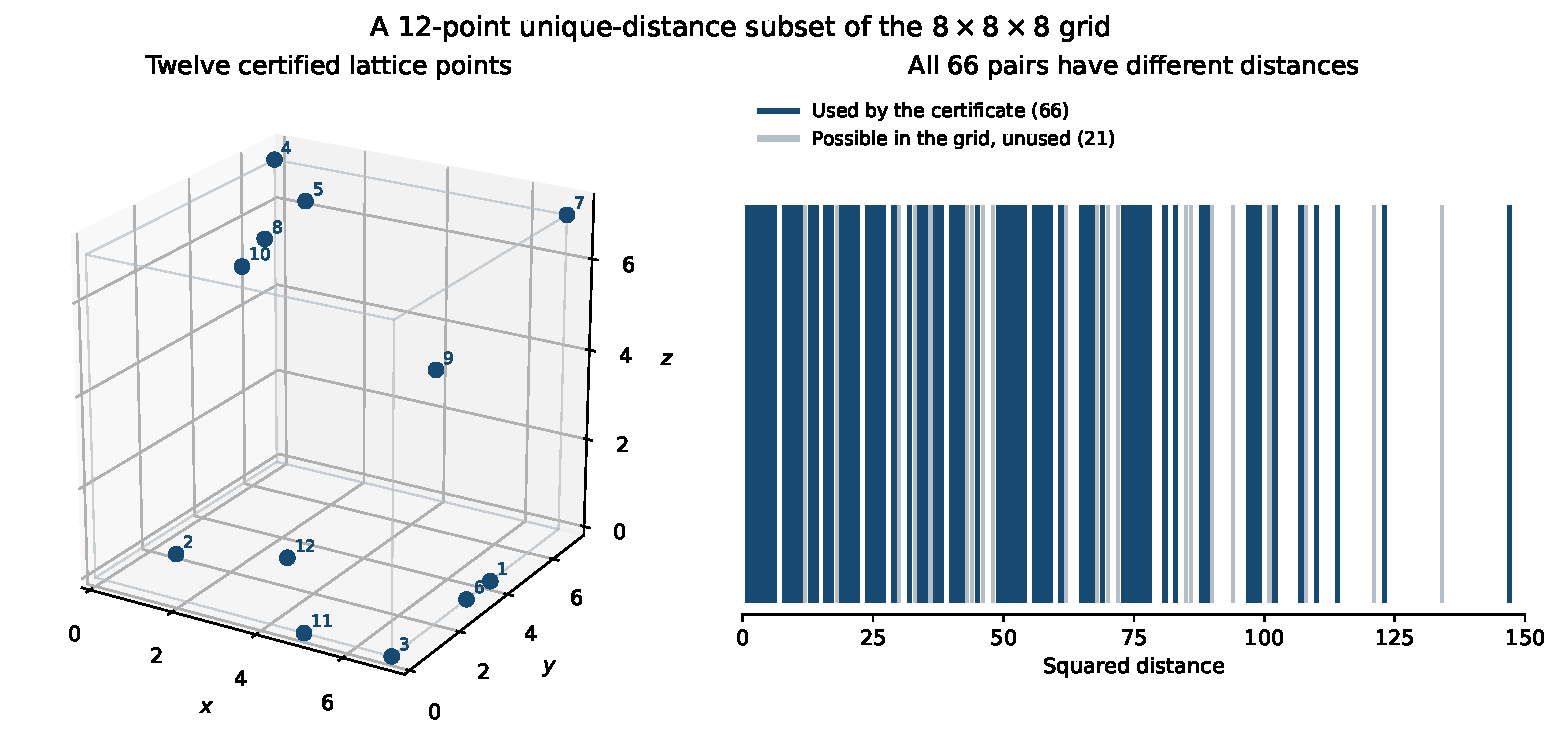
\includegraphics[width=\textwidth]{figures/witness_n8.pdf}
\caption{The 12-point witness in \(G_8\), with its exact squared-distance
spectrum. Gray marks are available cube distances that the witness does
not use. The 66 blue marks correspond to its 66 unordered pairs.}
\label{fig:witness}
\end{figure}
\[
\begin{aligned}
A_9=\{&(8,7,8),(4,0,2),(0,0,8),(2,0,8),\\
      &(8,8,0),(8,8,8),(4,8,0),(0,2,6),\\
      &(2,5,1),(3,4,2),(5,0,8),(3,3,1),(0,1,1)\}.
\end{aligned}
\]
The set \(A_9\) has 13 points and 78 distinct squared distances.
\[
\begin{aligned}
A_{10}=\{&(6,9,0),(9,3,6),(9,9,0),(0,0,1),\\
        &(1,0,9),(0,9,4),(9,8,1),(8,3,6),\\
        &(2,1,8),(7,7,0),(2,5,9),(6,0,9),\\
        &(9,8,3),(3,7,0)\}.
\end{aligned}
\]
The set \(A_{10}\) has 14 points and 91 distinct squared distances.

\subsection{A search that walks through valid configurations}
Collision-minimization searches found configurations with only one or
two repeated distances, but several stalled there. A more successful
procedure maintains a valid \(k\)-point set throughout. Delete three
points, or four with probability one third, leaving a fixed core. List
all grid points that are individually admissible against that core,
shuffle their order, and recursively refill while preserving distinctness.
A refill with one extra point proves a larger lower bound. An unsuccessful
bounded traversal can select a valid refill of the original size as the
next state.

This is a heuristic exploration of valid sets; a node cap limits each
move. The validity of every completed construction is exact, whereas
failure of a bounded traversal has no global meaning. With \(C\le n^3\)
remaining candidates and a traversal cap of \(B\) successful partial
refills, a safe per-move bound is \(O(n^3k+BCk)\). Counting only successful
partial refills does not count all failed candidate trials, so a claimed
\(O(Bk)\) bound would be unjustified.

The three displayed witnesses were found from valid starting sets in
497902, 109517, and 5858 moves respectively, with seeds 888112, 999123,
and 101314. Recorded wall times were approximately 108.75, 20.41,
and 1.29 seconds. These are warm-started search observations, not a
controlled comparison of algorithms or machines. The starting sets,
source code, and discovery metadata are included in the package.
A later version deletes four or five points per move. It produced
16 points in \(G_{12}\) and 18 points in \(G_{14}\), completing the
certified inequality \(a_n\ge n+4\) for every \(8\le n\le14\).
The immutable starting configurations and exact iteration budgets
for these runs are included as well.

\subsection{Certificate checks}
A separate Python verifier checks coordinate ranges, distinct points,
and a dictionary from squared distance to its unique unordered point
pair. It also verifies the full supplied distance inventory. Such a
check takes \(O(k^2)\) exact arithmetic operations for a witness of
size \(k\). No comparison of rounded Euclidean lengths is used.

\subsection{The complete finite catalogue through side length thirty}
All lower bounds in Table~\ref{tab:catalogue} have explicit coordinate
certificates. The upper bounds shown there are the elementary palette
and parity bounds; no exactness is asserted for these larger sizes.
\begin{table}[ht]
\centering
\caption{Certified bounds beyond side length ten. All point lists are supplied.}
\label{tab:catalogue}
\begin{tabular}{rrr@{\qquad}rrr}
\toprule
\(n\)&Lower&Upper&\(n\)&Lower&Upper\\
\midrule
11&15&19&21&22&38\\
12&16&21&22&23&40\\
13&17&23&23&24&42\\
14&18&24&24&25&43\\
15&18&26&25&26&46\\
16&18&28&26&26&48\\
17&19&30&27&27&50\\
18&20&32&28&28&52\\
19&21&34&29&29&54\\
20&22&36&30&30&55\\
\bottomrule
\end{tabular}
\end{table}

